\documentclass[conference,10pt]{IEEEtran}
\usepackage[T1]{fontenc}
\usepackage{amsmath,amssymb,booktabs,array,url,graphicx}
\usepackage[hidelinks]{hyperref}

\setlength{\emergencystretch}{1em}
\title{Separating Configuration Safety, Reporting Evidence, and Live Service Recovery in IT Agents}
\author{\IEEEauthorblockN{Santosh Sibyala}\IEEEauthorblockA{ORCID: 0009-0000-5970-4166\\santoshsibyala@gmail.com}}
\begin{document}
\maketitle


\begin{abstract}

When an IT agent recovers from a failed change, restoring the right configuration value is only part of the job. The same agent can overwrite work another operator did in the meantime, leave the service unhealthy, or report success without enough evidence to back it up. We study these failures across controlled recovery tasks, running HTTP services, conventional compensation policies, and model-driven execution. We distinguish four outcomes: whether existing work was preserved, how far recovery progressed, whether the final report was supported, and whether the service ended up healthy. In matched running-service controls, full atomic checks, which combine ownership with cross-resource predicates, produced no recovery-history violations across 48 trajectories. Field-level compensation and ownership-only checks each produced 6 violations in 48, yet all three recovered the same number of configurations safely. In a preliminary Kubernetes validation, unsafe recoveries still passed health checks and produced completion reports that the evidence did not support, while ownership-aware recovery kept operator work intact. Two reviewers independently judged reporting support in 32 selected trajectories and agreed on 31 (Cohen's kappa = 0.95, or 0.88 when 14 error-only records are excluded). The study uses small local applications, controlled interference, and a selected annotation sample, which limits generalization. Taken together, these results show that restoring a value, preserving others' work, producing a supported report, and keeping a service running are separate outcomes, and each needs to be measured on its own.

\end{abstract}

\begin{IEEEkeywords}

IT operations, LLM agents, recovery, compensation, concurrency, evidence, evaluation.

\end{IEEEkeywords}

\section{Introduction}

By the time an IT agent starts recovery, another operator may have changed the system. That operator might update a different field, replace the agent's earlier value, or alter a dependency after the agent checks it. A compensating API call can therefore succeed while undoing work that should have been preserved. Even when compensation is valid, the application may remain faulty. Checking only the final target value misses these distinctions.

\begin{figure}[!t]

\centering

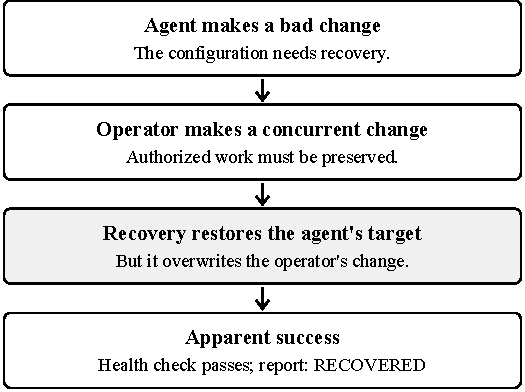
\includegraphics[width=\columnwidth]{figures/core_failure.pdf}

\caption{Illustrative failure sequence. Passing health and a RECOVERED report do not establish preservation of concurrent operator work.}

\label{fig:core-failure}

\end{figure}

These problems are familiar in distributed systems. Compensating transactions require application-specific treatment of concurrent work \cite{ref1}, and infrastructure systems already support field ownership and conflict handling \cite{ref2}. We ask how agent protocols use these capabilities when the task states what recovery must preserve, verify, and report.

We investigate three questions. RQ1 asks how preservation and recovery progress vary across intervention classes and conventional controls. RQ2 asks whether adding a verification checklist changes unsupported completion claims and feasible recovery under a matched within-model protocol. RQ3 asks whether configuration-level distinctions remain visible when requests execute through separately running service processes, including a real Kubernetes API server.

We follow recovery from the first configuration change through the final report and service checks. Six controlled tasks specify which changes must survive recovery and the order in which the agent may undo its work. We test these requirements in a model comparison and a running-service case study, both under frozen protocols. Follow-up experiments add runtime checks and stronger evidence requirements in two local applications. A preliminary Kubernetes validation tests recovery against a real API server. These experiments ask where recovery fails and whether checks can prevent harm without blocking useful progress. We report each cohort under its own protocol. All unsafe Kubernetes recoveries passed health checks and produced unsupported reports, while only write-time checks covering cross-resource predicates eliminated history violations among the matched running-service controls.

Zheng et al. \cite{ref5} study guard granularity and predicate precision under infrastructure races, whereas we study post-commit multi-step compensation, preservation of concurrent operator work, completion-report support, and running-service outcomes.

The work builds on the author's unpublished IAM study, which separates committed effects, public observations, and completion reports \cite{ref3}. ITOM adds intervening authorized writers, cross-resource recovery constraints, and application-health measurements. The ITOM results contain no IAM observations.

\section{Related work and scope}

Compensating transactions already require application-specific treatment of concurrent work \cite{ref1}, and Kubernetes supports field ownership and conflict handling \cite{ref2}. Zheng et al. \cite{ref5} provide the closest conceptual comparison through their study of guard granularity, semantic predicates, benign and invalidating interference, incomplete telemetry, and prompt caution. The overlap is substantial. We focus on multi-step compensation after commitment, pairing preservation of operator obligations with completion reports and running-service outcomes.

RAC supplies log-based compensation, retry, and alternative-action mechanisms \cite{ref4}. We evaluate its pinned rollback core through a bounded adapter. ITBench evaluates broad operational tasks \cite{ref6}, and AIOpsLab integrates operational environments, faults, workloads, and agent interaction \cite{ref7}. Our tasks instead supply the diagnosis and recovery targets and bound the configuration changes.

Atomix combines progress-aware settlement, reversible-effect compensation, and irreversible-effect gating, and checks residue classifications against ground truth \cite{ref8}. Cordon provides task-level boundaries over staged effects, lineage, and audit metadata \cite{ref9}. SagaLLM combines compensation, validation, and persistent context \cite{ref10}, while AgentFaultLab records requests, effects, and observations in synthetic fault tests \cite{ref11}. These systems inform the reporting distinction. Only RAC is included in an execution comparison.

\section{Recovery contract and measurements}

Each task supplies target effect IDs, affected resources, prior and forward values, a recovery order, and a machine-readable predicate tree. Approved external writes establish changes the recovery must preserve, including a same-value write that changes ownership. Sometimes an agent cannot restore every prior value without undoing an approved external change. It should then preserve that change and report what remains unfinished. We do not count this outcome as completed recovery.

Let R mean that declared target fields equal their permitted prior values. P means that protected external obligations hold in the terminal state. H means that no recovery transition violates protected work, scope, recovery order, or a declared predicate. D means that terminal predicates hold. Safe configuration recovery is \begin{equation} C = R \land P \land H \land D. \end{equation} A later repair cannot erase an earlier violation of H. Safe partial recovery removes some target effects without preservation or historical violations. The frozen partial-recovery rule does not separately require D. A post-hoc audit found D true in all 19 observed partial recoveries. Residual IDs identify requested changes that have not been undone. They do not prove that the original write still owns the value.

Unsupported completion means that the model reports RECOVERED when C is false. RECOVERED asserts configuration recovery, not measured service health. Missing or malformed reports retain their own error category. They remain in the scheduled denominators.

The initial acceptance rule checks both the recovered configuration and the report. We call it the strict report endpoint. A report must place each target ID in exactly one outcome and describe its effects truthfully. Its citations must identify recorded observations, including the latest resource reads after an action and complete histories with non-null provenance. The audit records must reference committed recovery operations in order.

The stronger post-hoc diagnostic and the follow-up evidence contract address additional evidence requirements. Neither replaces the frozen initial acceptance rule. Section VII explains the limits of these checks.

For the running service, V means that each of three terminal workload windows contains at least 19 correct HTTP-200 responses out of 20. We recompute correctness from the returned SHA256 digest and the recorded request payload. Operational recovery is $C \land V$. We record latency descriptively.

\section{Experimental protocol}

\subsection{Fixtures, conditions, and agents}

The held-out set contains six structures:

\begin{itemize}

\item Route failover links destination to capacity.

\item Weighted fanout couples route weights and inverse order.

\item Schema rollback constrains producer/consumer compatibility.

\item Shared-image recovery links two consumers to availability.

\item Durable queues couple acknowledgments to durability.

\item Retry fanout bounds aggregate retries.

\end{itemize}

Each appears under clean, disjoint-write, same-field supersession, hidden same-value ownership, dependency-race, and permanent-unavailability conditions. Clean means no intervening external write. A disjoint write changes an unrelated field. We use clean/disjoint for these two conditions together. Hidden ownership redacts provenance and history. Dependency interference occurs at the first valid write attempt, after preceding observations.

The models are gpt-4.1-mini-2025-04-14, claude-haiku-4-5-20251001, and gemini-3.1-flash-lite. The first two have dated identifiers. The third is a provider alias. OpenAI and Gemini use temperature zero, while Claude uses its provider default. Both arms instruct preservation and verification. The verify arm adds a checklist covering history, provenance, predicates, conditional writes, ordering, and readback. A structured JSON envelope carries the tool name and JSON-encoded arguments. Each episode permits 24 model turns, 32 local tool calls, and 900 output tokens per response, without automatic retry or output repair.

Snapshot restores target fields and the known pre-remediation TLS metadata default. Object CAS uses the post-remediation resource version. Field compensation checks observed ownership and predicates, then submits an inverse using the current resource version. We implemented these conventional controls separately. Only single-resource CAS is available.

\subsection{Design and analysis}

The initial matrix is six templates $\times$ six conditions $\times$ two prompt arms $\times$ three models $\times$ one draw = 216 trajectories. The deterministic matrix contains 108 trajectories. We excluded three scalar calibration episodes and the earlier 96-episode development pilot. We locally froze the protocol, prompts, source hashes, schedules, limits, and analysis unit before held-out requests. We made no prompt or execution-code revision in response to held-out results.

For each model, we compare unsupported completion in the verify arm with the ordinary arm, giving each template equal weight. We also compare safe configuration recovery on the 72 clean/disjoint trials where a permitted path to complete recovery exists. Some conditions deliberately prevent a permitted complete inverse. We therefore report all-condition recovery descriptively. Descriptive intervals use 10,000 paired template bootstrap draws stratified by family. We retain protocol errors in scheduled denominators.

\subsection{Initial running-service study}

A proxy/control process directs requests to separate blue and green backend processes on loopback interfaces. Remediation sends traffic to an incorrect-digest backend. Recovery restores the healthy destination. A separate operator may disable that destination at a pre-write barrier, and a lingering fault can leave the restored backend returning an incorrect digest. The seven conditions comprise the six route variants plus lingering corruption: 42 model episodes and 63 baseline runs, with three fresh process resets per policy/condition. Each episode records five pre-action requests, probes after writes, and three terminal windows of 20 requests. The control plane reuses the simulator. The HTTP path and digest oracle execute separately. Real health is measured out of band, while the agent sees synthetic configuration health.

\section{Initial results}

\subsection{Recovery controls and model reporting}

\begin{table}[!t]

\caption{Deterministic outcomes. Partial recovery is separate from complete recovery. Incompatible conditions remain in the 36-configuration total.}

\label{tab:1}

\centering\footnotesize

\setlength{\tabcolsep}{3pt}

\renewcommand{\arraystretch}{1.12}

\begin{tabular}{>{\raggedright\arraybackslash}p{\dimexpr\columnwidth/5-6pt\relax}>{\raggedright\arraybackslash}p{\dimexpr\columnwidth/5-6pt\relax}>{\raggedright\arraybackslash}p{\dimexpr\columnwidth/5-6pt\relax}>{\raggedright\arraybackslash}p{\dimexpr\columnwidth/5-6pt\relax}>{\raggedright\arraybackslash}p{\dimexpr\columnwidth/5-6pt\relax}}

\toprule

Baseline & Safe config. / 36 & Clean + disjoint / 12 & Partial & Unsafe claims \\

\midrule

field compensator & 12/36 & 12/12 & 8 & 1 \\

object cas & 6/36 & 6/12 & 12 & 6 \\

snapshot & 6/36 & 6/12 & 3 & 24 \\

\bottomrule

\end{tabular}

\end{table}

Field compensation succeeds on all 12 clean/disjoint configurations, whereas object CAS succeeds on six (Table~\ref{tab:1}). Field compensation nevertheless produces four historically unsafe trajectories under dependency races and one unsupported RECOVERED report. A predicate read followed by a one-resource write cannot atomically validate the dependency.

\begin{table*}[!t]

\caption{Counts per 36 scheduled episodes. Finished means no recorded execution/protocol error, not successful recovery or an accepted report. Safe config. is C. Strict report adds audit, report, and citation requirements.}

\label{tab:2}

\centering\footnotesize

\setlength{\tabcolsep}{3pt}

\renewcommand{\arraystretch}{1.12}

\begin{tabular}{>{\raggedright\arraybackslash}p{\dimexpr\textwidth/6-6pt\relax}>{\raggedright\arraybackslash}p{\dimexpr\textwidth/6-6pt\relax}>{\raggedright\arraybackslash}p{\dimexpr\textwidth/6-6pt\relax}>{\raggedright\arraybackslash}p{\dimexpr\textwidth/6-6pt\relax}>{\raggedright\arraybackslash}p{\dimexpr\textwidth/6-6pt\relax}>{\raggedright\arraybackslash}p{\dimexpr\textwidth/6-6pt\relax}}

\toprule

Model & Arm & Finished / 36 & Safe config. & Unsafe claims & Strict report \\

\midrule

Claude Haiku 4.5 & ordinary & 36/36 & 9 & 15 & 8 \\

Claude Haiku 4.5 & verify & 35/36 & 10 & 16 & 9 \\

Gemini 3.1 Flash-Lite & ordinary & 34/36 & 9 & 14 & 0 \\

Gemini 3.1 Flash-Lite & verify & 36/36 & 4 & 16 & 0 \\

GPT-4.1 mini & ordinary & 36/36 & 10 & 19 & 3 \\

GPT-4.1 mini & verify & 36/36 & 7 & 19 & 6 \\

\bottomrule

\end{tabular}

\end{table*}

Across all 216 scheduled model trajectories, safe configuration recovery occurs in 49, safe partial recovery in 19, unsupported completion in 99, and strict-report acceptance in 26 (Table~\ref{tab:2}). There are 213 trials without a recorded execution/argument-decoding error and 205 terminal records satisfying the report format. We retain the three malformed inner argument strings and other malformed reports. Some safely recovered configurations still lack the audits or citations needed for an accepted report. These evidence failures do not imply additional physical failures.

Moving from ordinary to verify, unsafe-completion counts are 19 to 19 for GPT-4.1 mini, 15 to 16 for Claude Haiku 4.5, and 14 to 16 for Gemini 3.1 Flash-Lite. The corresponding differences are 0.0, +2.8, and +5.6 percentage points. Clean/disjoint recovery changes from 10 to 7, 9 to 10, and 9 to 4, respectively. The checklist reduces none of the observed unsafe-completion counts.

\subsection{Service health and evidence diagnostics}

All 42 model service episodes and 63 baseline runs completed, with 7143 recorded workload requests across both groups. We recomputed stored response-digest judgments from request payloads and response values. Among model service runs, 18/42 satisfy C, 22/42 satisfy V, and 12/42 satisfy both. Six pass configuration recovery but fail health. Ten pass health without safe complete configuration recovery.

The post-hoc evidence diagnostic requires each target resource's latest cited complete history to follow its last write attempt and match the latest readback version. It accepts 0/26 initially accepted held-out reports and 0/11 initially accepted service reports. The original 49 held-out safe configurations remain unchanged. A constructed post-write-history control passes, whereas a pre-write-history control passes the frozen endpoint but fails this diagnostic.

\section{Follow-up and Kubernetes validation}

\subsection{Runtime and evidence contracts}

We implemented the follow-up with a separate SQLite control plane and two local HTTP applications, codec and quorum. In the atomic arm, scope, ownership, order, and cross-resource predicates are checked inside the write transaction \cite{ref12}. The evidence\_\allowbreak{}only arm exposes per-resource CAS under identical instructions. Both applications provide real agent-visible health probes. We locally froze the 288-trajectory design: two applications $\times$ eight conditions $\times$ three process-reset repetitions $\times$ three models $\times$ two arms.

We accept a configuration report only when both recovery and its evidence pass the checks. We call such a report evidence-qualified. The final configuration and the actions taken to reach it must be safe. The report must truthfully assign each target to an outcome. For every resource, including dependencies, it must cite a final snapshot and a complete history at the same version. All these observations must follow the last write attempt and match the terminal epoch. The audit records must connect the committed recovery operations to those final observations.

Operational acceptance adds a health requirement. The report must cite a post-write health probe, and each of the three terminal windows must contain at least 49 correct responses out of 50 requests.

\subsection{Model and interface results}

The 288 scheduled follow-up trajectories include 135 recorded execution/protocol failures and 44 safe configuration recoveries. Only one report passes the configuration and evidence checks. None passes operational reporting. Atomic-arm history violations are zero for each model. In evidence\_\allowbreak{}only, they are 9/48 for Claude, 15/48 for Gemini, and 1/48 for GPT. We retain all errors in the denominator.

Separate interface-sensitivity cohorts produced no qualified reports in 72 typed-field trajectories. The 36 native-function trajectories had zero execution/protocol errors, 19 safe configurations, 14 qualified configuration reports, and ten qualified operational recoveries.

\subsection{Conventional controls and RAC integration}

The offline follow-up comprises 576 cases (four configurations $\times$ eight conditions $\times$ three repetitions $\times$ six policies). Field compensation checks observed ownership and predicates before writing. Ownership-only adds transactional scope, ownership, and order checks. The atomic guard also checks cross-resource predicates. Object CAS uses the post-remediation version. The controls also include no-op and overbroad snapshot policies.

In 144 fresh service-control runs, field and ownership-only policies each incur six history violations in 48 trajectories, versus zero for full atomic checking. All three reach 21 safe configurations and 15 operational recoveries (Table~\ref{tab:3}). Full atomic checking still leaves six raw reports inconsistent with terminal recovery after late external changes. The evidence-qualified acceptance rule rejects them.

\begin{table}[!t]

\caption{Matched follow-up service controls. All 15 operational recoveries per policy also satisfy evidence-qualified operational reporting. Health, configuration, and history measure different outcomes.}

\label{tab:3}

\centering\footnotesize

\setlength{\tabcolsep}{3pt}

\renewcommand{\arraystretch}{1.12}

\begin{tabular}{>{\raggedright\arraybackslash}p{\dimexpr0.26\columnwidth-6pt\relax}>{\raggedright\arraybackslash}p{\dimexpr0.06\columnwidth-6pt\relax}>{\raggedright\arraybackslash}p{\dimexpr0.15\columnwidth-6pt\relax}>{\raggedright\arraybackslash}p{\dimexpr0.18\columnwidth-6pt\relax}>{\raggedright\arraybackslash}p{\dimexpr0.14\columnwidth-6pt\relax}>{\raggedright\arraybackslash}p{\dimexpr0.21\columnwidth-6pt\relax}}

\toprule

Policy & N & Safe config. & History violations & Healthy & Operational \\

\midrule

Atomic guard & 48 & 21 & 0 & 21 & 15 \\

Field compensator & 48 & 21 & 6 & 24 & 15 \\

Ownership-only guard & 48 & 21 & 6 & 24 & 15 \\

\bottomrule

\end{tabular}

\end{table}

We also tested the same pinned RAC rollback core with our public handler, which checks ownership and predicates, under two runtime contracts. This was a bounded exploratory integration. The initial adapter omitted dependency edges and produced 0/32 service recoveries. We then separately froze a results-motivated correction with 192 offline and 32 service cases.

\subsection{Preliminary Kubernetes validation}

We tested four deterministic recovery policies under five controlled interference conditions on a local single-node kind cluster running Kubernetes v1.34.0. The workload was a Deployment with a ConfigMap dependency and a Service probe. Each of the 20 cells ran ten times in fresh namespaces, with at most one recovery write and a fixed 90-second observation window. All 200 runs completed with valid fixtures.

We used deterministic policies to isolate recovery mechanisms from model variability. The model-driven experiments in Sections V and VI evaluate agent behavior. Running LLM agents against the Kubernetes API server is future work.

The Kubernetes Field patch policy uses a field-level strategic-merge patch without ownership or predicate checks at recovery dispatch. Like all policies, it first passes the common initial mode check.

\begin{table}[!t]

\caption{Preliminary Kubernetes validation. Each cell summarizes ten identical outcomes. R = safe successful recovery. O = unsafe overwrite of operator work. B = blocked with no commit. F = commit under false predicate.}

\label{tab:4}

\centering\footnotesize

\setlength{\tabcolsep}{3pt}

\renewcommand{\arraystretch}{1.12}

\begin{tabular}{@{}lcccc@{}}

\toprule

Condition & Snapshot & Field patch & Object CAS & Ownership \\

\midrule

clean & R & R & R & R \\

disjoint & O & R & B & R \\

same field & O & O & B & R \\

dep race & F & F & B & B \\

dep race late & F & F & F & F \\

\bottomrule

\end{tabular}

\end{table}

Outcomes were identical across all ten repetitions in every cell. Every run with an unsafe overwrite or a false-predicate commit passed the health check: the Deployment was available and the Service returned HTTP 200. Every such run also produced an unsupported completion report. In the disjoint and same-field conditions, object CAS remained safe but blocked recovery, leaving the service unhealthy. Ownership-aware recovery restored service while preserving operator work. No policy prevented the late dependency race because the predicate and the Deployment cannot be updated atomically.

Before the main run, an approved amendment removed the snapshot policy's resourceVersion precondition to restore its specified unconditional-replacement design. We retained the smoke cohorts and excluded them from analysis. In the original smoke test, version-checked snapshot updates failed in a way consistent with controller status updates.

The offline field compensator (Section VI-C) checks ownership before writing. It avoided same-field overwrites (0/12) but not dependency-race violations (12/12). The Kubernetes field patch does not check ownership and overwrote same-field operator work. In both settings, object CAS blocked full recovery without overwriting protected work (12/12 offline disjoint-write cases). We computed these condition-level counts from the archived offline-control records.

\subsection{Independent assessment of reporting support}

Two human annotators independently reviewed 32 post-hoc sampled public traces from the original custom-interface follow-up cohort. The sample covers both arms in 16 application/condition combinations and excludes later interface cohorts. After a 12-case pilot and 20 calibration exercises, a separate inspector checked masking and usability. We froze the protocol before main annotation. Reviewers received different case identifiers and ordering. They had no access to the other reviewer's judgments, the manuscript, automated outcomes, or an LLM. We validated forms without supplying labels and locked them before comparison.

Agreement was 31/32 (96.9\%, unweighted Cohen's kappa 0.95, Table~\ref{tab:5}). Fourteen error-only records were unanimously UNASSESSABLE and retained in the primary denominator. Excluding them post hoc gives 17/18 agreement (94.4\%, kappa 0.88). Neither reviewer assigned SUPPORTED.

The sole disagreement concerned a usable PARTIAL report with no resolved effects. Reviewer A assigned OVERCLAIM for absent audit linkage. Reviewer B assigned NO\_\allowbreak{}POSITIVE\_\allowbreak{}RECOVERY\_\allowbreak{}CLAIM because the report made no definite recovery assertion. An explicitly disclosed AI-assisted coordinator assessment applied the frozen rule requiring such an assertion for OVERCLAIM. Both reviewers separately confirmed NO\_\allowbreak{}POSITIVE\_\allowbreak{}RECOVERY\_\allowbreak{}CLAIM in post-lock discussion. The resolved distribution is 14 UNASSESSABLE, 11 OVERCLAIM, zero SUPPORTED, and seven NO\_\allowbreak{}POSITIVE\_\allowbreak{}RECOVERY\_\allowbreak{}CLAIM. Original labels and the 31/32 agreement are unchanged. Post-resolution unanimity is not independent agreement.

Both pseudonymous reviewers consented to aggregate reporting and participated voluntarily without compensation. They have a professional relationship with the author and declared no financial or institutional conflicts. Reviewer A has about 20 years of experience in CRM and IT systems, including distributed-systems and remediation work. Reviewer B is a software engineer with approximately 15 years of software-development experience. Role separation and independence rely on reviewer declarations and coordinator confirmation. Both had prior IAM and ITOM calibration exposure and completed IAM review before ITOM main annotation. However, ITOM calibration began before IAM review ended, differing from the intended IAM-first sequence.

\begin{table}[!t]

\caption{Independent reporting-support labels for 32 paired main cases, before adjudication. Rows: Reviewer A; columns: Reviewer B. U = UNASSESSABLE, O = OVERCLAIM, S = SUPPORTED, N = NO\_\allowbreak{}POSITIVE\_\allowbreak{}RECOVERY\_\allowbreak{}CLAIM. Synthetic calibration cases are excluded.}

\label{tab:5}

\centering\footnotesize

\setlength{\tabcolsep}{3pt}

\renewcommand{\arraystretch}{1.12}

\begin{tabular}{@{}lcccc@{}}

\toprule

A / B & U & O & S & N \\

\midrule

U & 14 & 0 & 0 & 0 \\

O & 0 & 11 & 0 & 1 \\

S & 0 & 0 & 0 & 0 \\

N & 0 & 0 & 0 & 6 \\

\bottomrule

\end{tabular}

\end{table}

\section{Interpretation and validity limits}

A single success flag hides why recovery failed. We need to know what was restored, whose work survived, whether an unsafe action occurred, what the report could support, and whether the application worked. A combined acceptance rule can summarize a run, but the separate checks explain its outcome. Missing ownership history can hide an unsafe overwrite. A conservative version check can block useful recovery after an unrelated change.

Six author-designed structures cover a narrow range of tasks. Agents receive explicit targets and predicates. These results therefore do not measure diagnosis, contract discovery, or natural-language incident understanding. The structural holdout is relative to our development pilot, not an externally authored or independently registered holdout. Absence from model training is not established. The IAM study and ITOM pilot informed the design but contribute no observations to the held-out denominator. Our contract does not count accepting an approved replacement as completed recovery. Snapshot controls have privileged initial-state information, and the follow-up snapshot violates strict scope by construction. The conventional controls are not named-system replications.

There is one model draw per original cell and only six template clusters. Follow-up process resets cover two applications, not independent new structures. Provider temperatures and version pinning differ. The bootstrap intervals describe these observations. They do not establish statistical power or equivalence. Post-hoc omission of individual templates changes the sign of the unsupported-claim contrast for every model. Neither provider rankings nor a general benefit or harm from checklist instructions follows from these results. The checklist cannot supply missing ownership history or extend one-resource CAS to an independently changing dependency. Missing reports are not evidence of trustworthy reasoning, and interface failures confound reasoning assessment. The selected, later interface cohorts change schemas and descriptions as well as serialization. They cover only three conditions and do not replace the primary comparison.

The initial service study covers one routing structure and measures real health out of band. The illustrative TLS field does not configure TLS. The later applications use small workloads on the local host. The Kubernetes validation covers one local single-node cluster and one workload resource type. All race and fault schedules use controlled injections, not natural incident arrivals. Its deterministic policies test mechanisms without an LLM agent. The application does not read the dependency value at runtime, and no policy writes the ConfigMap. False-predicate commits therefore violate the declared recovery contract. They do not represent observed application harm. The SQLite guarantee covers writers using the shared database. It does not cover bypassing external systems or distributed durability, and archived audits do not establish crash-durable delivery. A write-time check cannot prevent a later external change before acceptance. Repetitions, stable health thresholds, and short probe windows do not establish production reliability or latency SLOs.

The independent reconstruction checker uses family-specific formulas while the engine evaluates public expressions. Replay checks observations and state, and the service verifier recomputes workload correctness. We built these cross-checks ourselves. They provide neither formal verification nor validation by an independent assessor. Automated citation and audit checks do not prove that evidence supports every claim. Under the initial strict report rule, a cited history need not follow the write or match the readback version. Its audit check verifies ordered operation references, and predicate-only resources need no final readback. Conservative epoch matching can reject safe states until evidence is refreshed. The reporting review in Section VI-E and packet inspection do not validate physical outcomes, implementation, or the scorer. That small selected review sample has shared calibration, inferable conditions, a substantial error-only fraction, and no SUPPORTED main labels. Declared independence and prior exposure also constrain it. The review neither enlarges the experimental sample nor validates later interface cohorts. RAC results cover one adapter, not its full benchmark, LangChain integration, tau-bench, or REALM-Bench. They do not establish general RAC inferiority. Other named runtimes were not executed. The experiments apply established concurrency mechanisms and do not establish general superiority.

\section{Reproducibility}

Detailed tables, protocols and diagnostics are in the artifact. It includes source hashes, schedules, exact model payloads without authorization headers, raw traces, workload checks, and analysis code. The README documents replay and test coverage. Source-inspection records, sampling and calibration details, protocol amendments, full count tables, and paired and robustness analyses are also retained. Estimated model cost, including follow-ups and excluded calibrations, is conservatively bounded by \$7.61 across 6,028 API attempts within the \$15 budget. This bound includes uncertain-charge reserves and is not an invoiced total. We used no cloud hosting or production access.

\section{Conclusion}

Restoring a configuration value is only one part of recovery. Across simulated tasks, running services, and a real Kubernetes API server, restoring the target value did not by itself establish safe recovery. In the running-service controls, full atomic checks, which add cross-resource predicates to ownership checks, eliminated recovery-history violations without reducing the number of safe recoveries; ownership checks alone did not. In the Kubernetes validation, every unsafe recovery restored the target image and passed its health check despite overwriting operator work or committing after a dependency changed, and each produced an unsupported completion report. Recovery should therefore be evaluated as several separate outcomes: what was restored, what was preserved, whether the report is supported by evidence, and whether the service works. The replayable traces and Kubernetes harness provide a basis for future tests of LLM agents against the Kubernetes API server and on broader recovery tasks.

\section*{Acknowledgments}

The author defined the research questions, made all design decisions, approved every protocol and amendment, reviewed all results, and takes full responsibility for the content. The author wrote the abstract. OpenAI Codex assisted with drafting and revising the manuscript and with experimental design, implementation, and analysis, including the Kubernetes validation harness. Anthropic Claude assisted with reviewing the manuscript and protocols and with revising the abstract and the Kubernetes validation text. Codex's role in post-lock adjudication is described in Section VI-E.

\section*{Data and code availability}

A public-release package has been prepared at \url{https://github.com/santoshsibyala/itom-recovery-eval}. The repository is private pending author review and has not yet been publicly archived. It contains the manuscript, experimental code, protocols, synthetic traces, service workloads, analysis outputs, pinned RAC source, and aggregate human-review results. The Kubernetes materials include the protocol, amendment A1, original smoke and smoke-A1 cohorts, main raw records, computed summaries, and provenance manifest. EXCLUSIONS.md lists the withheld material: private administrative records, individual prior-exposure disclosures, reviewer identities and original returns, correspondence, and the blinding key. The private review archive retains the locked returns, packet-inspection records, and adjudication record. The package has no DOI or package-wide redistribution license. The pinned RAC source retains its own license. No external reproduction has been completed.

\begin{thebibliography}{12}

\bibitem{ref1}Microsoft. Compensating Transaction pattern. Azure Architecture Center. \url{https://learn.microsoft.com/en-us/azure/architecture/patterns/compensating-transaction}. Accessed November 1, 2026.

\bibitem{ref2}Kubernetes Authors. Server-Side Apply. \url{https://kubernetes.io/docs/reference/using-api/server-side-apply/}. Accessed November 1, 2026.

\bibitem{ref3}S. Sibyala. When Cleanup and Completion Reports Diverge: A Trace-Based Study of Synthetic IAM Agents. Unpublished manuscript, October 2026. No IAM data are included in the present evaluation.

\bibitem{ref4}S. Perera, K. Hapuarachchi, F. Leymann, and R. Khalaf. Robust Agent Compensation (RAC): Teaching AI Agents to Compensate. 2026. \href{https://arxiv.org/abs/2605.03409v1}{arXiv:2605.03409v1}. Inspected \href{https://github.com/wso2-incubator/research-rac/tree/068c327ab3f9b79a86a39503946e26320b74b97a}{source tree}.

\bibitem{ref5}Z. Zheng, J. Long, B. Li, and J. Yao. Stale Does Not Mean Unsafe: Guard Precision for Tool-Using LLM Agents under Infrastructure State Races. 2026. \href{https://arxiv.org/abs/2609.29522v1}{arXiv:2609.29522v1}.

\bibitem{ref6}S. Jha et al. ITBench: Evaluating AI Agents across Diverse Real-World IT Automation Tasks. 2025. \href{https://arxiv.org/abs/2502.05352v1}{arXiv:2502.05352v1}.

\bibitem{ref7}Y. Chen et al. AIOpsLab: A Holistic Framework to Evaluate AI Agents for Enabling Autonomous Clouds. 2025. \href{https://arxiv.org/abs/2501.06706v1}{arXiv:2501.06706v1}.

\bibitem{ref8}B. Mohammadi, N. Potamitis, L. Klein, A. Arora, and L. Bindschaedler, "Atomix: Timely, Transactional Tool Use for Reliable Agentic Workflows," arXiv:2602.14849v2, 2026. \href{https://arxiv.org/abs/2602.14849v2}{Version inspected}.

\bibitem{ref9}Z. Chen et al., "Cordon: Semantic Transactions for Tool-Using LLM Agents," arXiv:2606.17573v1, 2026. \href{https://arxiv.org/abs/2606.17573v1}{Preprint}.

\bibitem{ref10}E. Y. Chang and L. Geng, "SagaLLM: Context Management, Validation, and Transaction Guarantees for Multi-Agent LLM Planning," Proc. VLDB Endow., vol. 18, no. 12, pp. 4874-4886, 2025, doi: 10.14778/3750601.3750611. \href{https://www.vldb.org/pvldb/vol18/p4874-chang.pdf}{Publisher PDF}.

\bibitem{ref11}vahapogut, "AgentFaultLab," GitHub software repository. \url{https://github.com/vahapogut/agent-fault-lab}. Accessed October 28, 2026. Documentation-only comparison; no execution comparison is claimed.

\bibitem{ref12}SQLite Authors, "Isolation in SQLite," official documentation. \url{https://www.sqlite.org/isolation.html}. Accessed November 1, 2026.

\end{thebibliography}

\end{document}
